\section{Handover Trees}\label{sec.handover}

Before we start, we must introduce a small modification to the underlying proof-of-stake system
so that our protocol can be supported.

The proof-of-stake system proceeds in epochs. Consider an epoch $j$ and its slots
$S_j$, where $|S_j| = \mathcal{R}$. The slots
$S_j[-6k{:}]$ have leaders each of whom has
a public key. Call this sequence of keys $\overline{pk}_j$.
Since both the randomness $\eta_{j+1}$ and the stake
snapshot $\textsf{SD}_{j+1}$ are available during $S_j[-6k{:}]$, the $6k$ slot
leaders of epoch $j+1$ can already be deduced during $S_j[-6k{:}]$.
We require the following addition to the proof-of-stake protocol: Any block $b$
produced during the slots $S_j[-6k{:}-4k]$ \emph{must} include:

\begin{itemize}
  \item $b.\sigma$: A \emph{handover} signature by its leader on the plaintext consisting
        of the set of keys $\overline{pk}_{j+1}$.
  \item $b.\eta$ The randomness $\eta_{j+1}$ of the next epoch.
  \item $b\textsf{.SD}$ A Merkle tree commitment to the stake distribution snapshot $\mathsf{SD}_j$ to be used
        for the leader election of the next epoch.
  \item $b\textsf{.leaders}$ A Merkle tree commitment to the slot leaders of the whole chain,
        obtained according to the distribution and randomness up to and including
        epoch $j+1$.
\end{itemize}

These requirements are checked when the block is validated and before it is
extended by honest parties. We call $b.\sigma$
the \emph{handover} signature\footnote{Some practical blockchain systems
already implement similar handover signatures~\cite{nearbridge,horizon}.},
because it signifies a leader of epoch $j$ handing over
control to the $6k$ last leaders of epoch $j+1$.
These handover signatures will allow us to perform succinct proof-of-stake
synchronization. The last three of these data are only helpful for learning
more information about the current epoch once its leaders have been determined,
and may be omitted depending on the application. The $b\textsf{.leaders}$
structure contains all slot leaders\footnote{This is not an unusual structure
even for proof-of-work. For example, ZCash has already adopted such a structure,
and Ethereum has an approved proposal~\cite{eip210} for adopting it.}
from the beginning of time to allow for
checking of any transaction in the past. Since these are organized in a Merkle tree,
there is no harm to asymptotic performance.  If not all history is needed in practice,
this can be optimized to store only the leaders of the current $(j)$ and next $(j+1)$
epoch.

The public keys corresponding to the slots $S_j[-6k{:}-4k]$ are
the ones who will be responsible for providing signatures in their
blocks. We denote $\overline{pk}^*_j$ the sequence of these public keys
(this can be directly obtained by taking the first elements of $\overline{pk}_j$).

Because the stake and randomness used
in the next epoch leader election is uniquely
determined by all honest parties in consensus, all honest parties during
$S_j[-6k{:}-4k]$ will provide signatures over the \emph{same} plaintext
$\overline{pk}_{j+1}$. Of course, adversarial slot leaders may provide a signature
to a different plaintext or even generate multiple conflicting signatures.
By the \emph{honest subsequence} lemma, if
any $k+1$ among $\overline{pk}^*_j$
are chosen, there will exist at least one
honest key among them (since $|\overline{pk}^*_j| = 2k$ and they correspond to consecutive
slots). If we collect and verify a set $\overline{\sigma}_j$ of $k+1$ signatures
each of which was created with a key corresponding to distinct (i.e., in a distinct
sequence position) key in the sequence $\overline{pk}^*_j$ agreeing on the same
plaintext $\overline{pk}_{j+1}$, we can be certain that
$\overline{pk}_{j+1}$ really does correspond to the last $6k$ leaders of epoch
$j+1$.

\begin{figure*}[h]
    \centering
    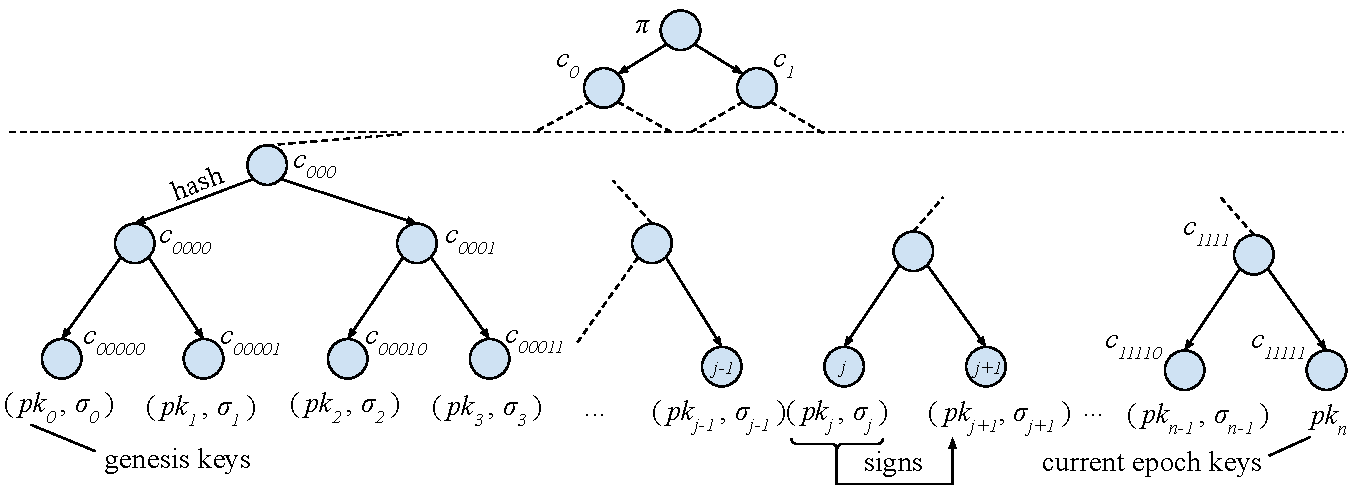
\includegraphics[width=0.8 \textwidth,keepaspectratio]{figures/popos-tree.pdf}
    \caption{The \emph{handover tree}, the central construction of our protocol.
             The root of the Merkle tree is the initial proof $\pi$. During the bisection
             game, the signatures between the challenge node $j$ and its neighbours
             $j-1$ and $j+1$ are validated.}
    \label{fig.popos-tree}
\end{figure*}

\import{./}{algorithms/alg.prover-tree}

We begin our construction by describing the first message exchanged between the
honest prover and the verifier during their interaction. The verifier initially
requests a \emph{proof} from each of the provers in $\mathcal{P}$. This proof
consists of three elements: The root $\pi$ of a Merkle tree; the claimed size
$n > 1$ of the Merkle tree's leaves.
The honest prover Merkle tree is constructed by creating \emph{one leaf per epoch}.
The $j^\text{th}$ leaf corresponds to the $j^\text{th}$ epoch. It consists of a pair of the sets
$(\overline{pk}_j, \overline{\sigma}_j)$, the a set
of public keys $\overline{pk}_j$ corresponding to $S_j[-6k{:}]$,
and a set of signatures $\overline{\sigma}_j$ handing over control to the next epoch $j+1$.
During verification we will require that, for every $j$, 
$|\overline{\sigma}_j| = k + 1$, and it will follow that
$|\overline{pk}_{j+1}| = 6k$.

The number of leaves in the Merkle tree are equal to the number of epochs in
the execution, and so will be $\lceil\frac{|\chain|}{\mathcal{R}}\rceil$.
Since $\mathcal{R} = 16k$ is a constant, this quantity is proportional to
$\chain$. If the tree were to be sent in full from the prover to the verifier,
this would harm succinctness, but these leaves are never all seen by the verifier.
Throughout the protocol's execution, only the
root of the tree and a small number of leaves, with their respective inclusion proof
paths, will be exchanged, to ensure succinctness. The number of leaves revealed will
be constant. Each inclusion proof path has a size of $\textsf{poly}\log n$, and so
our communication complexity will be logarithmic.

This \emph{handover tree} is illustrated in Figure~\ref{fig.popos-tree}.
Each node contains a set of public keys and a signature. The signature must verify
with the public keys in the same leaf. The signature must verify with the plaintext
consisting of the public keys in the next leaf. The first leaf in the tree must
have public keys $\overline{pk}_0$ corresponding to the last $6k$ slots of the
genesis epoch, whose stake distribution $\textsf{SD}_0$ and randomness $\eta_0$
are known from the genesis block $\mathcal{G}$. The last leaf is the only one
with a public key but not a signature, since we may have not yet obtained a handover
signature to the next epoch. The nodes are hashed together in pairs to obtain the
root $\pi$ of the binary tree.

The procedure for the creation of the tree root and its nodes appears in Algorithm~\ref{alg.prover-tree}.
The function $H$ denotes a cryptographically secure hash function.
The leaves of the tree are collected by the function \emph{get-handover}. Given a chain $\chain$,
the function iterates over each epoch $j$ in the chain. For each epoch, it observes the last $6k$ slots $S$.
For these, it extracts the sequence $pk[j]$ of the public keys of the leaders,
and the sequence $\sigma[j]$ of handover signatures,
which are verifiable using the public keys $pk[j]$ on the plaintext $pk[j+1]$. The sequence of public keys
and the sequence of signatures are both placed in
the array $d$ containing the final leaves. For the last epoch, only the public keys are collected,
since the signatures are not yet available.
The tree is constructed in a bottom-up fashion by the recursive function $\textsf{build-tree}(d, p)$,
which is invoked with the desired leaves $d$ and starting at depth $0$ with $p = \epsilon$.
The tree nodes are stored in the dictionary $T$. The keys in the dictionary are binary strings.
The key length indicates the depth of the node. The root lives at the key $\epsilon$ at depth $0$.
The left child of the root lives at $0$, while the right child of the root lives at $1$, both at depth $1$.
The left child of the left child of the root lives at $00$, and so forth. The left and right subtrees
are constructed recursively by setting an appropriate path prefix $p$. The left subtree contains
the leaves $d[{:}\textsf{mid}]$, while the right subtree contains the rest of the leaves
$d[{:}\textsf{mid}]$. The value \emph{mid} is calculated so that the count of the left subtree's leaves
is equal to the largest power of $2$ smaller than $|d|$. The right subtree contains whatever is
leftover\footnote{While not necessary for our protocol, structuring the tree in this manner
left-to-right instead of balancing it exactly makes it easier to append nodes to these trees\cite{ct}.}.
As such, the left subtree may have equal height to the right subtree, or the right subtree may have
a height of one less. Each intermediate node is the hash of its concatenated children.
Each leaf contains the hash of its value in $d$. We assume that the values in $d$ are distinct from
the outputs of $H$; this can be achieved by prefixing each node with a bit to indicate whether it
is a node whose value is given by the output of the hash, or a leaf node value that is not the output
of the hash.
